\documentclass[11pt,]{article}
\usepackage[left=1in,top=1in,right=1in,bottom=1in]{geometry}
\newcommand*{\authorfont}{\fontfamily{phv}\selectfont}
\usepackage[]{mathpazo}


  \usepackage[T1]{fontenc}
  \usepackage[utf8]{inputenc}



\usepackage{abstract}
\renewcommand{\abstractname}{}    % clear the title
\renewcommand{\absnamepos}{empty} % originally center

\renewenvironment{abstract}
 {{%
    \setlength{\leftmargin}{0mm}
    \setlength{\rightmargin}{\leftmargin}%
  }%
  \relax}
 {\endlist}

\makeatletter
\def\@maketitle{%
  \newpage
%  \null
%  \vskip 2em%
%  \begin{center}%
  \let \footnote \thanks
    {\fontsize{18}{20}\selectfont\raggedright  \setlength{\parindent}{0pt} \@title \par}%
}
%\fi
\makeatother




\setcounter{secnumdepth}{0}

\usepackage{color}
\usepackage{fancyvrb}
\newcommand{\VerbBar}{|}
\newcommand{\VERB}{\Verb[commandchars=\\\{\}]}
\DefineVerbatimEnvironment{Highlighting}{Verbatim}{commandchars=\\\{\}}
% Add ',fontsize=\small' for more characters per line
\usepackage{framed}
\definecolor{shadecolor}{RGB}{248,248,248}
\newenvironment{Shaded}{\begin{snugshade}}{\end{snugshade}}
\newcommand{\KeywordTok}[1]{\textcolor[rgb]{0.13,0.29,0.53}{\textbf{{#1}}}}
\newcommand{\DataTypeTok}[1]{\textcolor[rgb]{0.13,0.29,0.53}{{#1}}}
\newcommand{\DecValTok}[1]{\textcolor[rgb]{0.00,0.00,0.81}{{#1}}}
\newcommand{\BaseNTok}[1]{\textcolor[rgb]{0.00,0.00,0.81}{{#1}}}
\newcommand{\FloatTok}[1]{\textcolor[rgb]{0.00,0.00,0.81}{{#1}}}
\newcommand{\ConstantTok}[1]{\textcolor[rgb]{0.00,0.00,0.00}{{#1}}}
\newcommand{\CharTok}[1]{\textcolor[rgb]{0.31,0.60,0.02}{{#1}}}
\newcommand{\SpecialCharTok}[1]{\textcolor[rgb]{0.00,0.00,0.00}{{#1}}}
\newcommand{\StringTok}[1]{\textcolor[rgb]{0.31,0.60,0.02}{{#1}}}
\newcommand{\VerbatimStringTok}[1]{\textcolor[rgb]{0.31,0.60,0.02}{{#1}}}
\newcommand{\SpecialStringTok}[1]{\textcolor[rgb]{0.31,0.60,0.02}{{#1}}}
\newcommand{\ImportTok}[1]{{#1}}
\newcommand{\CommentTok}[1]{\textcolor[rgb]{0.56,0.35,0.01}{\textit{{#1}}}}
\newcommand{\DocumentationTok}[1]{\textcolor[rgb]{0.56,0.35,0.01}{\textbf{\textit{{#1}}}}}
\newcommand{\AnnotationTok}[1]{\textcolor[rgb]{0.56,0.35,0.01}{\textbf{\textit{{#1}}}}}
\newcommand{\CommentVarTok}[1]{\textcolor[rgb]{0.56,0.35,0.01}{\textbf{\textit{{#1}}}}}
\newcommand{\OtherTok}[1]{\textcolor[rgb]{0.56,0.35,0.01}{{#1}}}
\newcommand{\FunctionTok}[1]{\textcolor[rgb]{0.00,0.00,0.00}{{#1}}}
\newcommand{\VariableTok}[1]{\textcolor[rgb]{0.00,0.00,0.00}{{#1}}}
\newcommand{\ControlFlowTok}[1]{\textcolor[rgb]{0.13,0.29,0.53}{\textbf{{#1}}}}
\newcommand{\OperatorTok}[1]{\textcolor[rgb]{0.81,0.36,0.00}{\textbf{{#1}}}}
\newcommand{\BuiltInTok}[1]{{#1}}
\newcommand{\ExtensionTok}[1]{{#1}}
\newcommand{\PreprocessorTok}[1]{\textcolor[rgb]{0.56,0.35,0.01}{\textit{{#1}}}}
\newcommand{\AttributeTok}[1]{\textcolor[rgb]{0.77,0.63,0.00}{{#1}}}
\newcommand{\RegionMarkerTok}[1]{{#1}}
\newcommand{\InformationTok}[1]{\textcolor[rgb]{0.56,0.35,0.01}{\textbf{\textit{{#1}}}}}
\newcommand{\WarningTok}[1]{\textcolor[rgb]{0.56,0.35,0.01}{\textbf{\textit{{#1}}}}}
\newcommand{\AlertTok}[1]{\textcolor[rgb]{0.94,0.16,0.16}{{#1}}}
\newcommand{\ErrorTok}[1]{\textcolor[rgb]{0.64,0.00,0.00}{\textbf{{#1}}}}
\newcommand{\NormalTok}[1]{{#1}}
\usepackage{longtable,booktabs}

\usepackage{graphicx}
% We will generate all images so they have a width \maxwidth. This means
% that they will get their normal width if they fit onto the page, but
% are scaled down if they would overflow the margins.
\makeatletter
\def\maxwidth{\ifdim\Gin@nat@width>\linewidth\linewidth
\else\Gin@nat@width\fi}
\makeatother
\let\Oldincludegraphics\includegraphics
\renewcommand{\includegraphics}[1]{\Oldincludegraphics[width=\maxwidth]{#1}}

\title{Oil Price Volatility  }



\author{\Large James P. Hamski\vspace{0.05in} \newline\normalsize\emph{City University of New York}  }


\date{}

\usepackage{titlesec}

\titleformat*{\section}{\normalsize\bfseries}
\titleformat*{\subsection}{\normalsize\itshape}
\titleformat*{\subsubsection}{\normalsize\itshape}
\titleformat*{\paragraph}{\normalsize\itshape}
\titleformat*{\subparagraph}{\normalsize\itshape}


\usepackage{natbib}
\bibliographystyle{apsr}



\newtheorem{hypothesis}{Hypothesis}
\usepackage{setspace}

\makeatletter
\@ifpackageloaded{hyperref}{}{%
\ifxetex
  \usepackage[setpagesize=false, % page size defined by xetex
              unicode=false, % unicode breaks when used with xetex
              xetex]{hyperref}
\else
  \usepackage[unicode=true]{hyperref}
\fi
}
\@ifpackageloaded{color}{
    \PassOptionsToPackage{usenames,dvipsnames}{color}
}{%
    \usepackage[usenames,dvipsnames]{color}
}
\makeatother
\hypersetup{breaklinks=true,
            bookmarks=true,
            pdfauthor={James P. Hamski (City University of New York)},
             pdfkeywords = {oil price, commodities, time series analysis, volatility clustering},
            pdftitle={Oil Price Volatility},
            colorlinks=true,
            citecolor=blue,
            urlcolor=blue,
            linkcolor=magenta,
            pdfborder={0 0 0}}
\urlstyle{same}  % don't use monospace font for urls



\begin{document}

% \pagenumbering{arabic}% resets `page` counter to 1
%
% \maketitle

{% \usefont{T1}{pnc}{m}{n}
\setlength{\parindent}{0pt}
\thispagestyle{plain}
{\fontsize{18}{20}\selectfont\raggedright
\maketitle  % title \par

}

{
   \vskip 13.5pt\relax \normalsize\fontsize{11}{12}
\textbf{\authorfont James P. Hamski} \hskip 15pt \emph{\small City University of New York}   

}

}







\begin{abstract}

    \hbox{\vrule height .2pt width 39.14pc}

    \vskip 8.5pt % \small

\noindent Oil price volatility \ldots{}


\vskip 8.5pt \noindent \emph{Keywords}: oil price, commodities, time series analysis, volatility clustering \par

    \hbox{\vrule height .2pt width 39.14pc}



\end{abstract}


\vskip 6.5pt

\noindent \doublespacing \section{Acknowledgements}\label{acknowledgements}

\emph{I would like to thank John Kemp, Thompson Reuters energy
journalist, for posing the question investigated in this research paper.
In addition, I thank Tancred Lidderdale and Mason Hamilton from the U.S.
Energy Information Administration for additional information pertaining
to the question.}

\section{Introduction}\label{introduction}

In a commodity trading market the price level is expected to be tied to
the system dynamics. Volatility, the variation in price over time,
reflects uncertainty in the supply, demand, and delivery of the
commodity being traded. This research paper aims to answer a simply
posed question: ``does oil price volatility scale with price?''; i.e.,
can we expect to observe larger price swings when the price is near
\$100/barrel vs \$20/barrel?

If oil price volatility reflects uncertainty about supply and demand
dynamics, it isn't immediately clear whether we should expect volatility
to depend on price level. Higher oil prices are associated with
``tightness'' in the supply market, meaning there is little excess
capacity to increase production. However, factors such as storage
dynamics, the ability of producers to increase production fast enough to
bring more oil to market in response to high prices (``rebalancing''),
and market speculation complicate this picture and mean it must be
studied empirically.

If it is found that oil price volatility is dependent on price level,
the relationship may follow a scaling formula. For instance, if we can
expect volatility of \$1/barrel when oil is at \$20/barrel, can we
expect volatility of \$5/barrel at \$100/barrel price levels via a
simple linear scaling rule? Three methods are presented in this research
paper to answer this question: (1) regression modeling of price and
volatility, (2) viewing volatility within oil price regimes, and (3)
using multivariate Generalized Autoregressive Conditional
Heteroskedasticity (GARCH) modeling.

Note that in this research paper \emph{oil price} is used to
specifically mean spot-traded crude oil. This represents only one
component of the oil markets, and most of the actual oil price is
determined by futures and long term delivery contracts (need cite). This
research paper is concerned with understanding the energy system using
pricing information. In this way, it differs from much of the published
research in that it is not concerned with forecasting prices or
volatility. Nor is it addressing exogeneous system elements such as
equity markets or interest rates, though the literature shows that the
crude oil market and larger economic indicators are intertwined (add
cite). Instead, it contributes to our understanding of the system
dynamics of an essential energy commodity.

\begin{Shaded}
\begin{Highlighting}[]
\KeywordTok{library}\NormalTok{(broom)}
\KeywordTok{library}\NormalTok{(changepoint)}
\KeywordTok{library}\NormalTok{(knitr)}
\KeywordTok{library}\NormalTok{(magrittr)}
\KeywordTok{library}\NormalTok{(TSA)}
\KeywordTok{library}\NormalTok{(xts)}
\end{Highlighting}
\end{Shaded}

\begin{Shaded}
\begin{Highlighting}[]
\KeywordTok{load}\NormalTok{(}\StringTok{"wti_project.Rda"}\NormalTok{)}
\end{Highlighting}
\end{Shaded}

\section{Exploratory Data Analysis}\label{exploratory-data-analysis}

\subsection{Data Source}\label{data-source}

The data source is the West Texas Intermediate (WTI) nominal (i.e.~not
inflation adjusted) daily spot price record from the U.S. Energy
Information Administration. The WTI series was filtered to the date
range January 2, 1986 through December 30, 2016.

\begin{Shaded}
\begin{Highlighting}[]
\KeywordTok{summary}\NormalTok{(wti.xts) %>%}\StringTok{ }\KeywordTok{tidy}\NormalTok{()}
\end{Highlighting}
\end{Shaded}

\begin{verbatim}
##    Var1       Var2                 Freq
## 1            Index Min.   :1986-01-03  
## 2            Index 1st Qu.:1993-09-01  
## 3            Index Median :2001-06-11  
## 4            Index Mean   :2001-06-19  
## 5            Index 3rd Qu.:2009-03-31  
## 6            Index Max.   :2016-12-30  
## 7          wti.xts     Min.   : 10.25  
## 8          wti.xts     1st Qu.: 19.38  
## 9          wti.xts     Median : 28.01  
## 10         wti.xts     Mean   : 42.87  
## 11         wti.xts     3rd Qu.: 63.47  
## 12         wti.xts     Max.   :145.31
\end{verbatim}

\subsection{Returns and Volatility}\label{returns-and-volatility}

In this research paper, volatility is characterized two ways: (1) 5-day
historic volatility and (2) 30-day historic volatility. In addition, the
relationship between the returns themselves and price level is
investigated. Single-period returns were calculated as:
\[R_t = \frac{P_t-P_{t-1}}{P_{t-1}}\] and in some sections, their
absolute values are used.

\begin{Shaded}
\begin{Highlighting}[]
\KeywordTok{par}\NormalTok{(}\DataTypeTok{mfrow =} \KeywordTok{c}\NormalTok{(}\DecValTok{2}\NormalTok{, }\DecValTok{2}\NormalTok{))}
\KeywordTok{plot.xts}\NormalTok{(wti.xts, }\DataTypeTok{type =} \StringTok{"l"}\NormalTok{, }\DataTypeTok{ylab =} \StringTok{"Nominal Dollars ($)"}\NormalTok{, }\DataTypeTok{main =} \StringTok{"WTI Price Series"}\NormalTok{)}
\KeywordTok{plot.xts}\NormalTok{(wti.return, }\DataTypeTok{type =} \StringTok{"l"}\NormalTok{, }\DataTypeTok{main =} \StringTok{"WTI Return Series"}\NormalTok{)}
\KeywordTok{plot.xts}\NormalTok{(wti.combined[,}\DecValTok{3}\NormalTok{], }\DataTypeTok{type =} \StringTok{"l"}\NormalTok{, }\DataTypeTok{main =} \StringTok{"WTI 30-day Historic Volatility"}\NormalTok{)}
\KeywordTok{plot.xts}\NormalTok{(wti.combined[,}\DecValTok{4}\NormalTok{], }\DataTypeTok{type =} \StringTok{"l"}\NormalTok{, }\DataTypeTok{main =} \StringTok{"WTI 5-day Historic Volatility"}\NormalTok{)}
\end{Highlighting}
\end{Shaded}

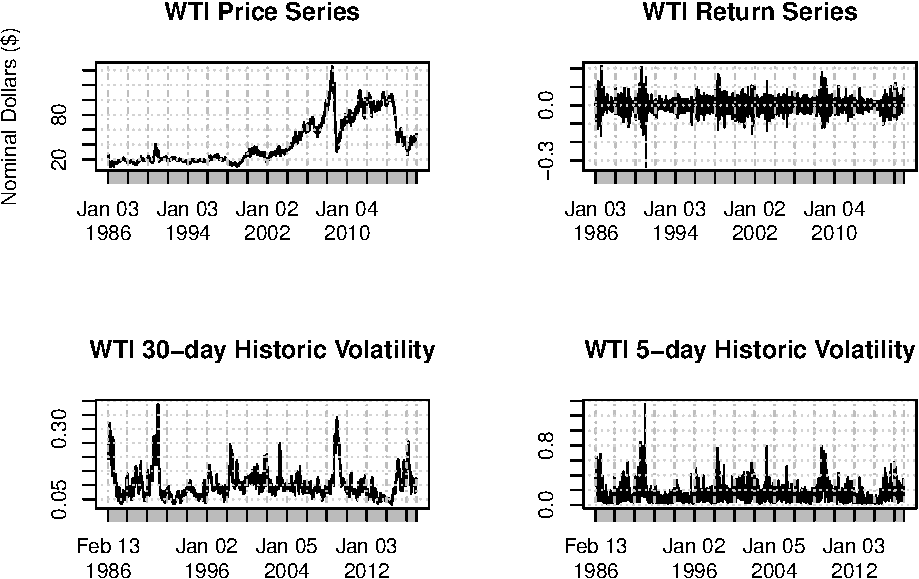
\includegraphics{JHamski_manuscript_files/figure-latex/unnamed-chunk-4-1.pdf}

Ase seen in Figure 1, most of the series from 1986 through 2004 contains
prices between \$10/barrel and \$40/barrel. This results in a price
series with left skew and a long right tail. These distribution
characteristics are common in financial time series. The return series
displays the

\begin{Shaded}
\begin{Highlighting}[]
\KeywordTok{par}\NormalTok{(}\DataTypeTok{mfrow =} \KeywordTok{c}\NormalTok{(}\DecValTok{1}\NormalTok{, }\DecValTok{2}\NormalTok{))}
\KeywordTok{plot}\NormalTok{(}\KeywordTok{density}\NormalTok{(wti.xts), }\DataTypeTok{main =} \StringTok{"Oil Prices Density Plot"}\NormalTok{, }\DataTypeTok{xlab =} \StringTok{"Dollars per Barrel"}\NormalTok{)}
\KeywordTok{curve}\NormalTok{(}\KeywordTok{dnorm}\NormalTok{(x, }\DataTypeTok{mean=}\KeywordTok{mean}\NormalTok{(wti.xts), }\DataTypeTok{sd=}\KeywordTok{sd}\NormalTok{(wti.xts)), }
          \DataTypeTok{col=}\StringTok{"darkblue"}\NormalTok{, }\DataTypeTok{lwd=}\DecValTok{1}\NormalTok{, }\DataTypeTok{add=}\OtherTok{TRUE}\NormalTok{, }\DataTypeTok{yaxt=}\StringTok{"n"}\NormalTok{)}

\KeywordTok{plot}\NormalTok{(}\KeywordTok{density}\NormalTok{(wti.return), }\DataTypeTok{main =} \StringTok{"Oil Returns Density Plot"}\NormalTok{, }\DataTypeTok{xlab =} \StringTok{"Dollars per Barrel"}\NormalTok{)}
\KeywordTok{curve}\NormalTok{(}\KeywordTok{dnorm}\NormalTok{(x, }\DataTypeTok{mean=}\KeywordTok{mean}\NormalTok{(wti.return), }\DataTypeTok{sd=}\KeywordTok{sd}\NormalTok{(wti.return)), }
          \DataTypeTok{col=}\StringTok{"darkblue"}\NormalTok{, }\DataTypeTok{lwd=}\DecValTok{1}\NormalTok{, }\DataTypeTok{add=}\OtherTok{TRUE}\NormalTok{, }\DataTypeTok{yaxt=}\StringTok{"n"}\NormalTok{)}
\end{Highlighting}
\end{Shaded}

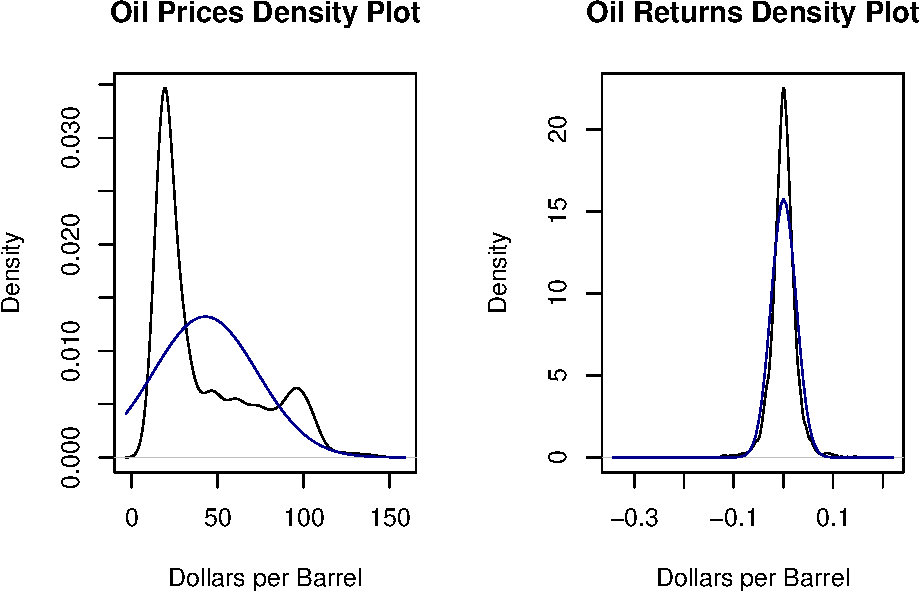
\includegraphics{JHamski_manuscript_files/figure-latex/unnamed-chunk-5-1.pdf}

Times series exploration

\begin{Shaded}
\begin{Highlighting}[]
\KeywordTok{par}\NormalTok{(}\DataTypeTok{mfrow =} \KeywordTok{c}\NormalTok{(}\DecValTok{1}\NormalTok{, }\DecValTok{2}\NormalTok{))}
\KeywordTok{acf}\NormalTok{(}\KeywordTok{abs}\NormalTok{(wti.return), }\DataTypeTok{lag.max =} \DecValTok{50}\NormalTok{)}
\KeywordTok{pacf}\NormalTok{(}\KeywordTok{abs}\NormalTok{(wti.return), }\DataTypeTok{lag.max =} \DecValTok{50}\NormalTok{)}
\end{Highlighting}
\end{Shaded}

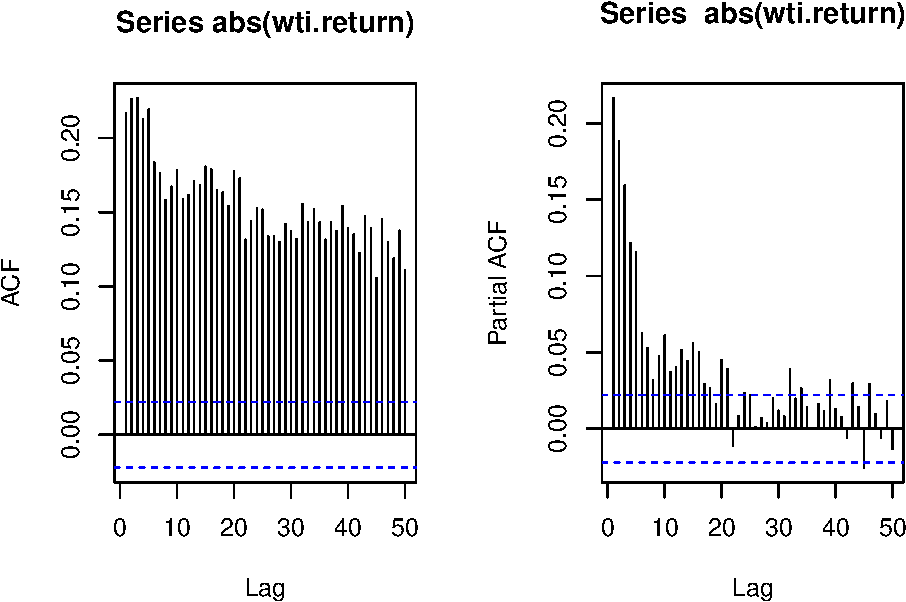
\includegraphics{JHamski_manuscript_files/figure-latex/unnamed-chunk-6-1.pdf}

A challenge in analyzing financial time series in general, and spot oil
market prices specifically, is that the variance structure may be
independent, but not identically distributed. Oil prices exhibit periods
of low volatility (i.e.~relatively constant prices) and periods of high
volatility (i.e.~changing prices). This is referred to as volatility
clustering. This violates the assumption in the most frequently used
time series model, the autoregressive integrated moving average (ARIMA)
model.

\begin{Shaded}
\begin{Highlighting}[]
\KeywordTok{McLeod.Li.test}\NormalTok{(}\DataTypeTok{y =} \NormalTok{wti.return)}
\end{Highlighting}
\end{Shaded}

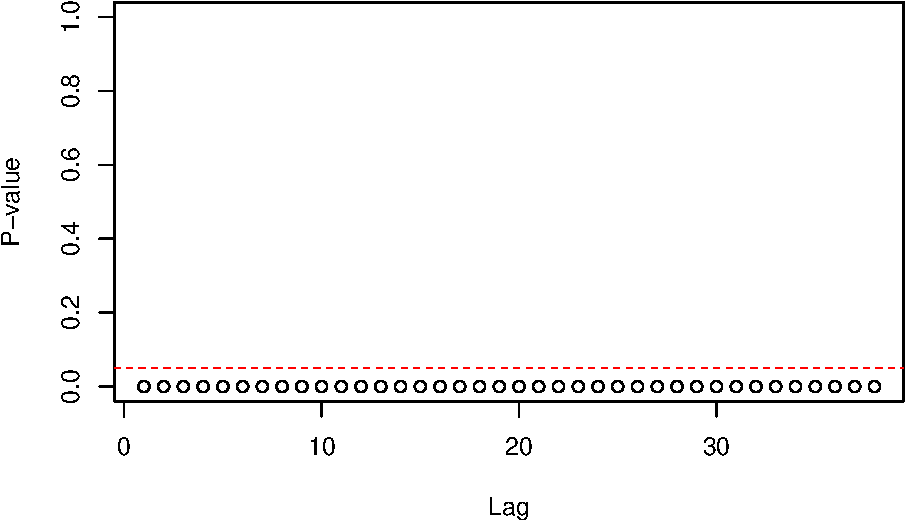
\includegraphics{JHamski_manuscript_files/figure-latex/unnamed-chunk-7-1.pdf}

\section{Price-Volatility Regression
Analysis}\label{price-volatility-regression-analysis}

\begin{Shaded}
\begin{Highlighting}[]
\NormalTok{cov.results <-}\StringTok{ }\KeywordTok{cov}\NormalTok{(wti.df)[}\DecValTok{1}\NormalTok{,}\DecValTok{2}\NormalTok{:}\DecValTok{4}\NormalTok{]}
\NormalTok{cor.results <-}\StringTok{ }\KeywordTok{cor}\NormalTok{(wti.df)[}\DecValTok{1}\NormalTok{,}\DecValTok{2}\NormalTok{:}\DecValTok{4}\NormalTok{]}

\NormalTok{cov.cor <-}\StringTok{ }\KeywordTok{cbind}\NormalTok{(cov.results, cor.results)}
\KeywordTok{colnames}\NormalTok{(cov.cor) <-}\StringTok{ }\KeywordTok{c}\NormalTok{(}\StringTok{"Covariance"}\NormalTok{, }\StringTok{"Correlation"}\NormalTok{)}
\KeywordTok{kable}\NormalTok{(cov.cor)}
\end{Highlighting}
\end{Shaded}

\begin{longtable}[]{@{}lrr@{}}
\toprule
& Covariance & Correlation\tabularnewline
\midrule
\endhead
return & -0.0396337 & -0.0719290\tabularnewline
30-day & -0.2933686 & -0.1864200\tabularnewline
5-day & -0.3757726 & -0.1212286\tabularnewline
\bottomrule
\end{longtable}

The case of 30-day historic volatility indicates a negative relationship
between price level and volatility. However, this result appears to be
due to a cluster high volatility around \$20/barrel, creating a leverage
point. Residual analysis indicates that this is not a good relationship
to model with linear regression.

\begin{Shaded}
\begin{Highlighting}[]
\NormalTok{returns.lm <-}\StringTok{ }\KeywordTok{lm}\NormalTok{(return ~}\StringTok{ }\NormalTok{close, }\DataTypeTok{data =} \NormalTok{wti.combined)}
\NormalTok{TD.lm <-}\StringTok{ }\KeywordTok{lm}\NormalTok{(}\StringTok{`}\DataTypeTok{30-day}\StringTok{`} \NormalTok{~}\StringTok{ }\NormalTok{close, }\DataTypeTok{data =} \NormalTok{wti.combined)}
\NormalTok{FD.lm <-}\StringTok{ }\KeywordTok{lm}\NormalTok{(}\StringTok{`}\DataTypeTok{5-day}\StringTok{`} \NormalTok{~}\StringTok{ }\NormalTok{close, }\DataTypeTok{data =} \NormalTok{wti.combined)}

\KeywordTok{plot}\NormalTok{(}\DataTypeTok{x =} \NormalTok{wti.df$close, }\DataTypeTok{y =} \NormalTok{wti.df$return) +}\StringTok{ }\KeywordTok{abline}\NormalTok{(returns.lm)}
\end{Highlighting}
\end{Shaded}

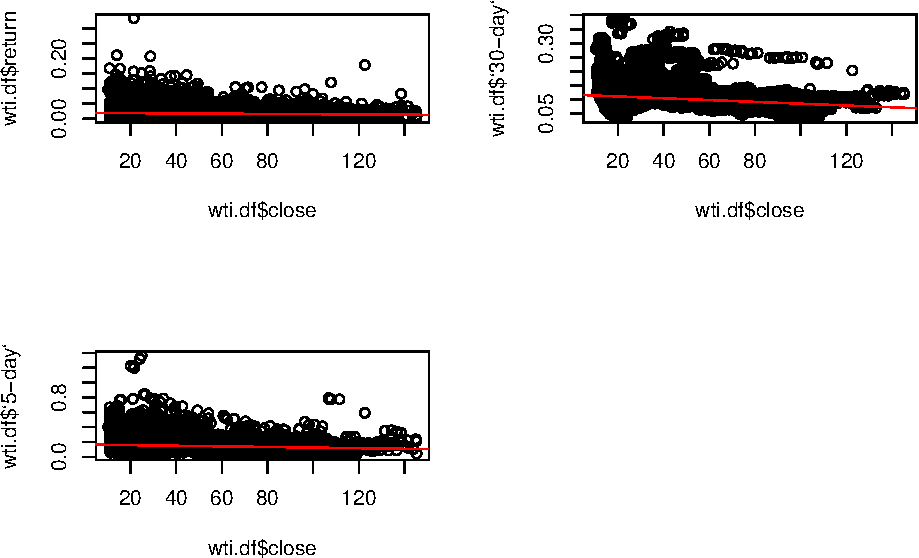
\includegraphics{JHamski_manuscript_files/figure-latex/unnamed-chunk-9-1.pdf}

\begin{verbatim}
## numeric(0)
\end{verbatim}

\begin{Shaded}
\begin{Highlighting}[]
\KeywordTok{plot}\NormalTok{(}\DataTypeTok{x =} \NormalTok{wti.df$close, }\DataTypeTok{y =} \NormalTok{wti.df$}\StringTok{`}\DataTypeTok{30-day}\StringTok{`}\NormalTok{) +}\StringTok{ }\KeywordTok{abline}\NormalTok{(TD.lm)}
\end{Highlighting}
\end{Shaded}

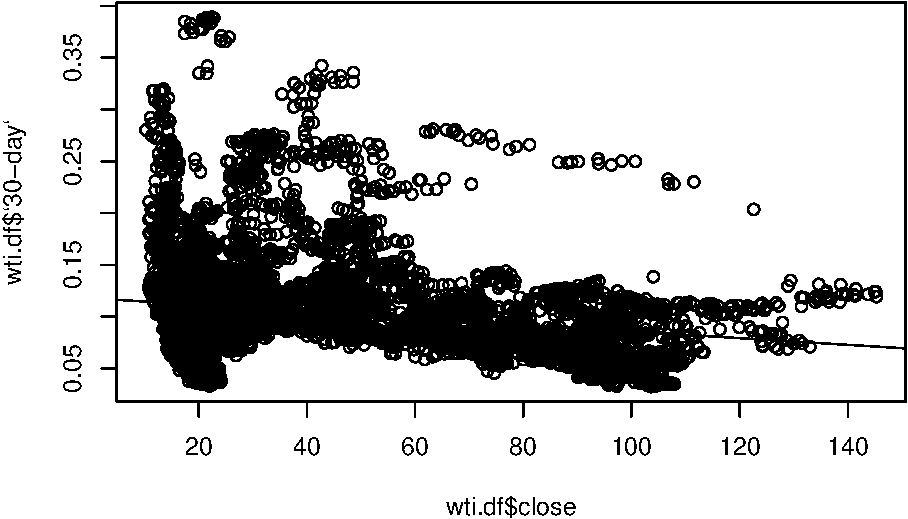
\includegraphics{JHamski_manuscript_files/figure-latex/unnamed-chunk-9-2.pdf}

\begin{verbatim}
## numeric(0)
\end{verbatim}

\begin{Shaded}
\begin{Highlighting}[]
\KeywordTok{plot}\NormalTok{(}\DataTypeTok{x =} \NormalTok{wti.df$close, }\DataTypeTok{y =} \NormalTok{wti.df$}\StringTok{`}\DataTypeTok{5-day}\StringTok{`}\NormalTok{) +}\StringTok{ }\KeywordTok{abline}\NormalTok{(FD.lm)}
\end{Highlighting}
\end{Shaded}

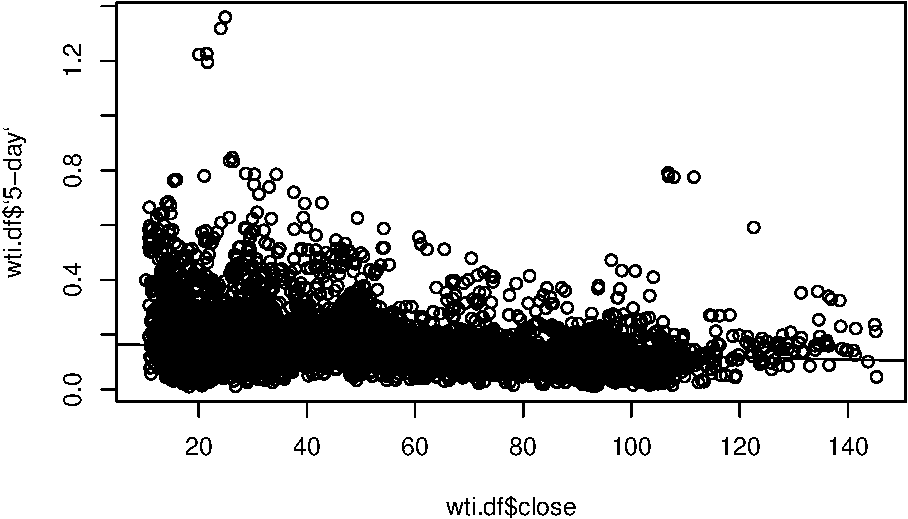
\includegraphics{JHamski_manuscript_files/figure-latex/unnamed-chunk-9-3.pdf}

\begin{verbatim}
## numeric(0)
\end{verbatim}

As seen in Figure 1, nominal oil prices have spent time as high as
\$145/barrel. However, the majority of the time series is far lower,
with a median price of \$28/barrel. This means that the dataset is
unbalanced and higher price levels represent a smaller portion of the
dataset. In addition, oil price (and financial time series in general)
exhibits volatility clustering. Therefore, it is anticipated that this
simple regression model based on price and volatility is not the best
possible solution to the question of characterizing the dependency of
volatility on price.

\section{Comparing Volatility across Price
Regimes}\label{comparing-volatility-across-price-regimes}

Changepoint detection aims to detect the point or points where the
statistical properties of a sequence of observations change (Killick and
Eckley, 2014). Changepoint detection was used to detect change in the
oil price mean throughout the period of record using the Pruned Exact
Linear Time (PELT) algorithm (Killick et al. 2012). The time series
between these changepoints represent ``price regimes'' (i.e.~time series
between changepoints) which have generally similar mean oil price
compared to the entire record.

Changepoint detection proceeds by minimizing a cost function over
possible locations and number of changepoints. The cost function:
\newpage
\singlespacing
\bibliography{master.bib}
\end{document}
